\subsection{Query Completion}
\label{sec:completion}

\begin{figure*}[t]
    \centering
    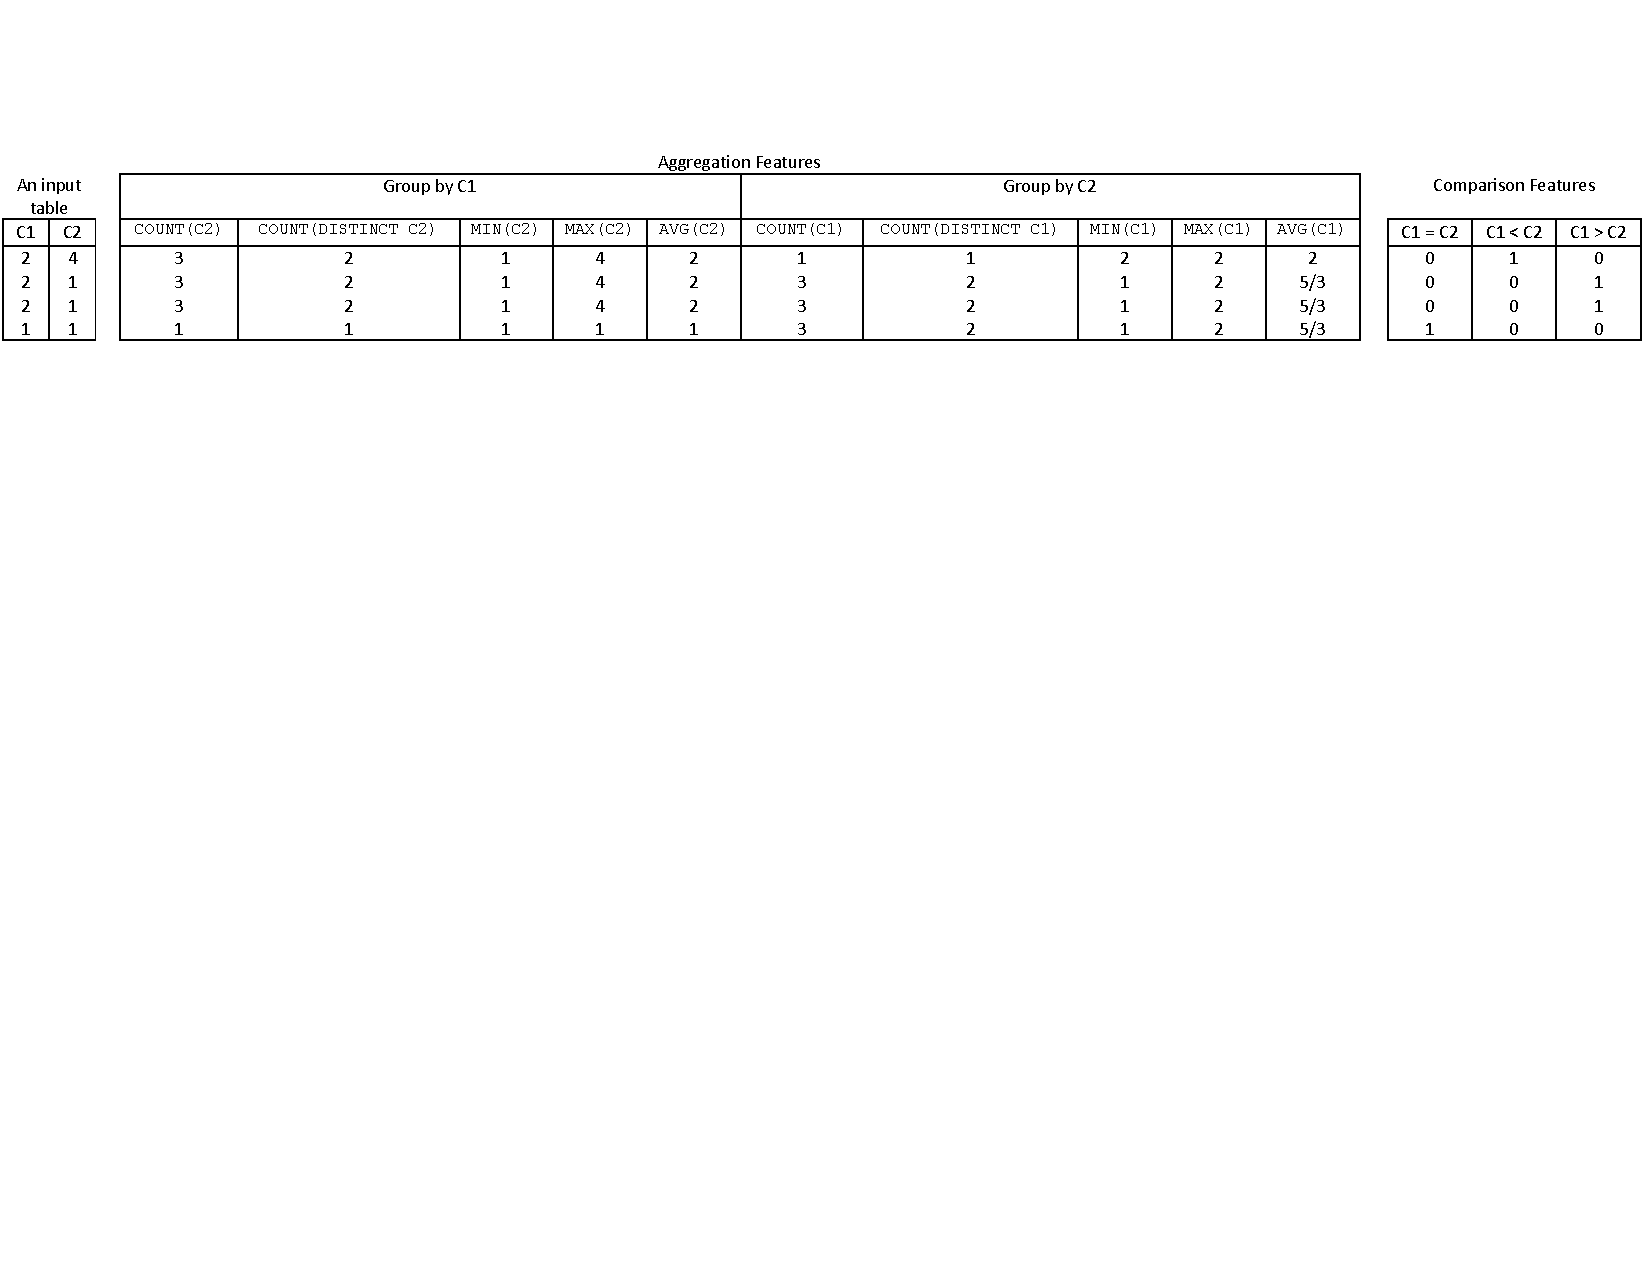
\includegraphics[scale=0.68]{featurex}
    \vspace{-7mm}
	\caption{Illustration of two additional features
    added by \ourtool. (Left) An example input table with
    two columns: C1 and C2. (Center) The aggregation features added by
    \ourtool for the input table. (Right) The comparison features
    added by \ourtool for the input table.
    Take the first row in the input table as an example,
    when grouping the table by column C1 (with value 2), the number
    of values in the C2 column is 3; the  number of
    distinct values in the C2 column is 2; the minimal value
    in the C2 column is 1, the maximal value in the C2 column
    is 4, and the average value in the C2 column is 2. Similar
    results can be computed if the table is grouped by the C2
    column.
}
	\label{fig:features}
\end{figure*}


In this step, \ourtool analyzes each created query skeleton
, and completes the missing query conditions, the
\CodeIn{GROUP BY} and \CodeIn{HAVING} clause (Section~\ref{sec:condition}),
aggregates (Section~\ref{sec:agg_search}), and
the \CodeIn{ORDER BY} clause (Section~\ref{sec:orderby}).
\ourtool outputs a list of syntactically-correct SQL queries
that satisfy the given example input and output.


%The SQL skeleton produced by the first step, though incomplete,
%serves as a good reference in inferring complete and valid SQL queries.
%In this step, our technique the remaining incomplete parts: conditions and
%aggregates, by rule-based learning and type-directed search, respectively.

\subsubsection{Inferring Query Conditions}
\label{sec:condition}

\ourtool casts the problem of \textit{inferring query conditions} as
 \textit{learning appropriate rules} that can perfectly divide a search space
into a positive part and a negative part. In our context, the search space
is all tuples from joining all query tables; the positive part
includes all tuples in the output table; and the negative part includes the rest
tuples.

The standard way for rule learning is using a decision-tree-based
algorithm. However, how to design a good features
becomes a key challenge.
Existing approaches~\cite{Tran:2009} simply use
tuple values in the input table(s) as features, 
and limits their abilities in inferring more
complex rules as query conditions. In particular,
merely using tuple values as features can only infer
conditions that compares a column value with a constant
(e.g., \CodeIn{student.level = 'senior'}), but
fails to infer conditions using aggregates (e.g., \CodeIn{COUNT(enrolled.course\_id) > 2}),
or conditions comparing the values of two table columns
(e.g., \CodeIn{enrolled.course\_id > enrolled.score}).



\ourtool addresses this challenge by adding two types of
additional features to each tuple, and uses
the existing tuple values together with the additional features
for rule learning.

\begin{itemize}

\item {\textbf{Aggregation Features}}. For each
column in an input table, \ourtool tries
to group all table data by \textit{each} tuple's
value, then applies every applicable aggregate (i.e.,
\CodeIn{COUNT}, \CodeIn{COUNT DISTINCT}, \CodeIn{MAX},
\CodeIn{MIN}, and \CodeIn{AVG} for a numeric type column;
and \CodeIn{COUNT}, and \CodeIn{COUNT DISTINCT} for
a string type column) to every
 \textit{remaining} column for computing the aggregation result. 
The ``Aggregation Features'' part in Figure~\ref{fig:features}
shows an example.

\item {\textbf{Comparison Features}}. For each tuple,
\ourtool compares
the values of every two type-comparable columns, and records
the comparison results ($1$ or $0$) as features.
The ``Comparison Features'' part in Figure~\ref{fig:features}
shows an example.

\end{itemize}

%The above two additional features seamlessly encodes SQL
%structure
% knowledge encoding permits our technique
%to make use of correlations between columns, rather than only values
%from each isolated and sequential columns.
%Table~\ref{tbl:com} shows an example.


%Using both tuple values and the enhanced features,
\ourtool employs a variant of the decision tree algorithm,
called PART~\cite{Frank:1998}, to learn a set of rules
as query conditions.
PART has two notable advantages over the
original decision tree algorithm~\cite{Quinlan:1986}.
First, it uses a ``divide-and-conquer'' strategy to repeatedly
build rules and remove data instances (i.e., tuples) that have already been covered until
no more data instances are left, and thus is faster.
Second, PART less memory, since it builds a decision
tree incrementally, prunes falsified branches on-the-fly,
and only keeps the minimal tree structure in memory.



\todo{The incerasing number of features, can be falsified quickly,
more features permits undiscover more rules}


Figure~\ref{fig:fullexample} shows an example, in
which the expected query condition uses the \CodeIn{COUNT} aggregate.


\begin{figure*}[t]
  \centering
  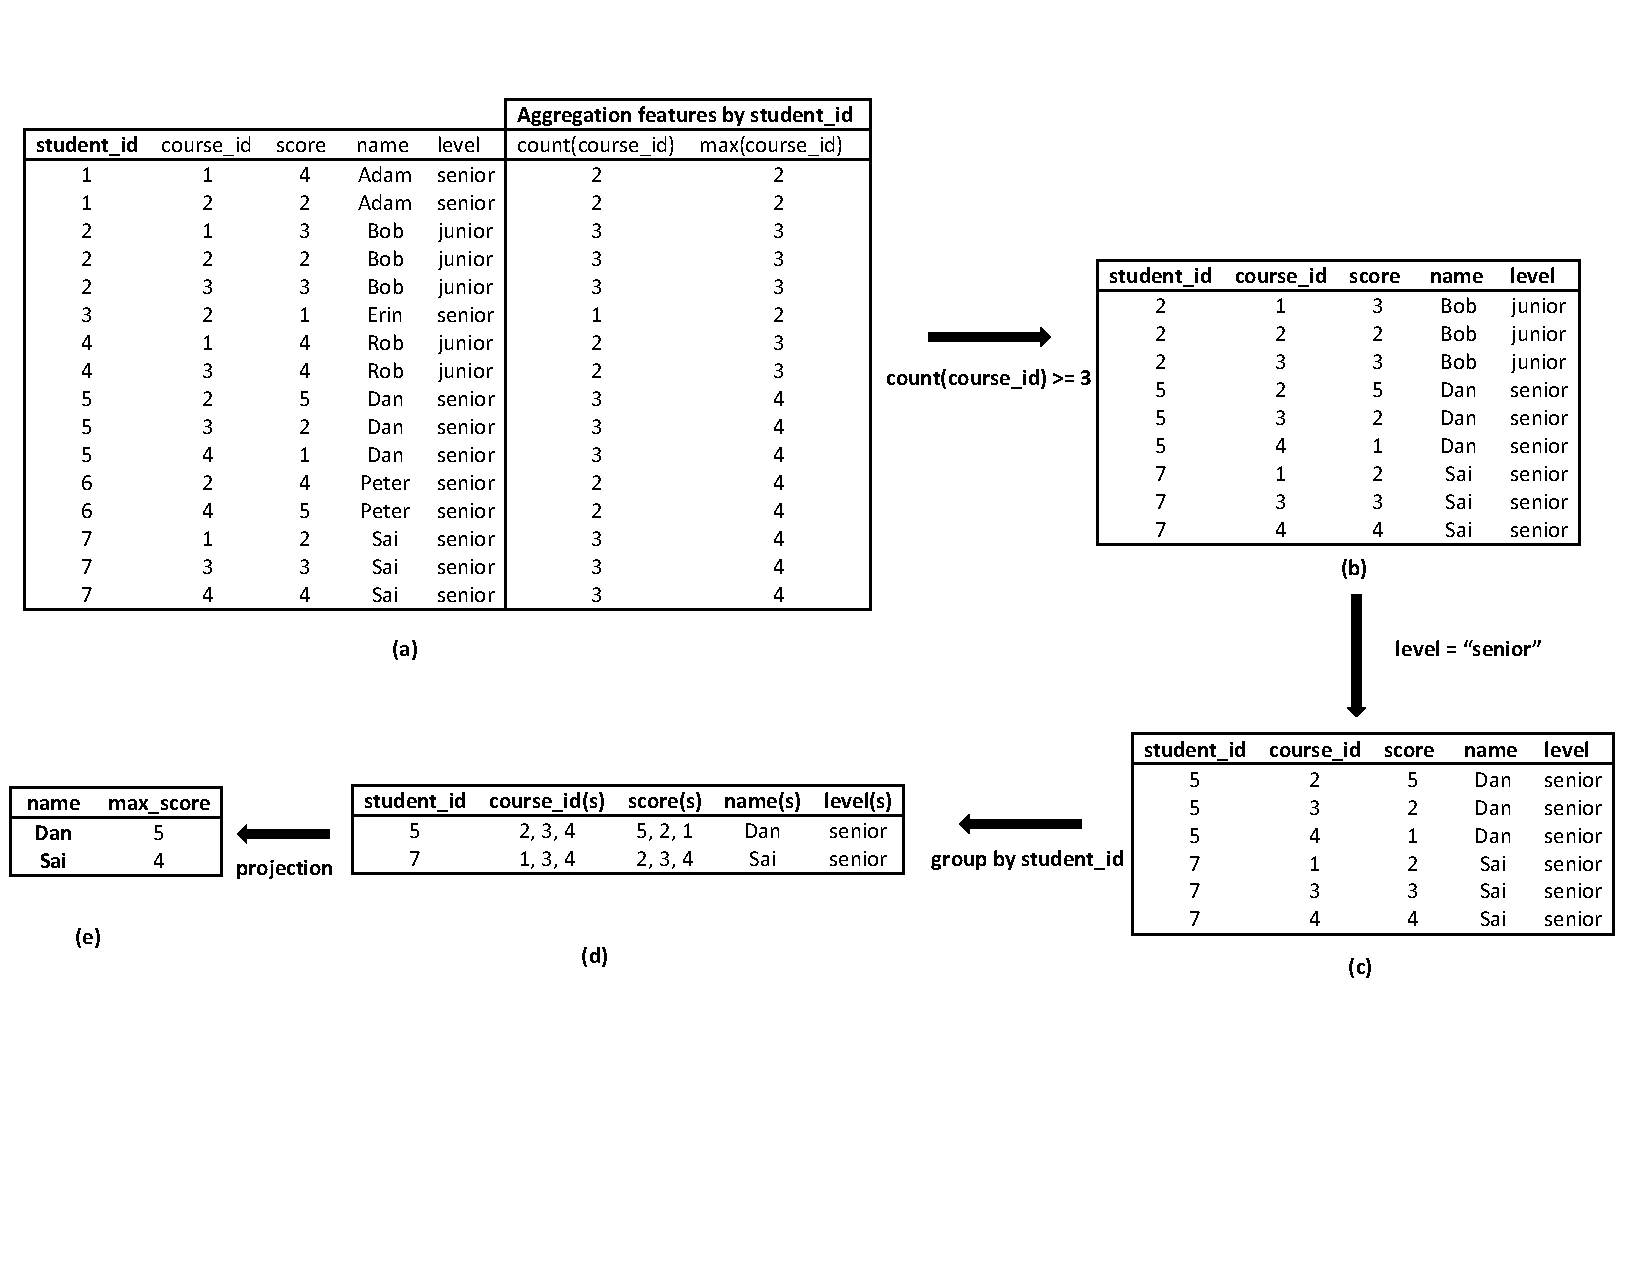
\includegraphics[scale=0.65]{fullexample}
  \vspace*{-5.0ex}\caption {{\label{fig:fullexample}
  Illustration of how additional features added by \ourtool
  helps in inferring query conditions. (a) shows \ourtool
  enriches the original table (Left: the
  result of joining table \CodeIn{student} with table
  \CodeIn{enrolled} on the \CodeIn{student\_id} column)
  with additional features. For brevity, only relevant
  aggregation features are shown. Using the added aggregation
  features, \ourtool infers two query conditions that
  transform the original table into the table show in (b).
  Note that, without the aggregation features enhanced by
  \ourtool, a learning algorithm will \textit{fail} to learn the above conditions.
  (c) shows the output table, which is produced by projecting the
   table in (b)
  on its column: name, and an aggregate: \CodeIn{MAX}(score).
}}

\end{figure*}


\ourtool next splits the learnt rules into two disjoint parts:
and put each part into its appropriate place.
Specifically, \ourtool puts conditions
using aggregates to the \CodeIn{HAVING}
clause; and puts other conditions to the \CodeIn{WHERE} clause.
This is based on the SQL language's specification:
query conditions using aggregates are valid only when they
are used \textit{after} the \CodeIn{GROUP BY} clause.
Take the conditions inferred in Figure~\ref{fig:fullexample}
as an example, \ourtool puts the query
condition: \CodeIn{student.level =`senior'}
in the \CodeIn{WHERE} clause,
puts condition: \CodeIn{COUNT(enrolled.course\_id) > 2}
in the \CodeIn{HAVING} clause, and puts
column \CodeIn{student\_id} to the \CodeIn{GROUP BY} clause.

%\smallskip





%\end{itemize}

\subsubsection{Searching for Aggregates}
\label{sec:agg_search}

For every column in the output table that has no matched
column in the input tables,
\ourtool repeatedly applies each aggregate on
every input table column; and then outputs the aggregate (with the
input table column) that produces the same output 
in the output table. To speed up the exhaustive search,
\ourtool uses two rules to filter away many infeasible
combinations.


\begin{itemize}
\item \ourtool only applies an \textit{applicable} aggregate
to a \textit{type-compatible} table column. Specifically,
the data values in an output column must be compatible with an
aggregator's return type. For instance, if an output column
contains float values, it cannot be produced by using the \CodeIn{COUNT}
or \CodeIn{COUNT DISTINCT} aggregators, or 
using the \CodeIn{MAX} aggregator over a column with integer type.
On the other hand, some aggregates cannot be applied on
table columns with certain types. For example, the \CodeIn{AVG}
aggregate cannot be applied to columns with string type.
%\ourtool encodes such knowledge to avoid unnecessary search.

\item \ourtool checks whether each value in the output
column has appeared in the input table. If not, the
output column cannot be produced by using
using the \CodeIn{MAX} and \CodeIn{MIN} aggregator.
%such as \CodeIn{MAX} and \CodeIn{min},
%is used, each value in the output column must has appeared in the input table.
\end{itemize}

%In our experience, the type-directed searching strategy significantly reduces the
%searching space and makes our tool find the desirable aggregates faster.

%\todo{Order by structure, relatively each to add}
\subsubsection{Searching for columns in the \CodeIn{ORDER BY} column}
\label{sec:orderby}
\ourtool scans the values of each column in the output table. If
the data values in a column are sorted, \ourtool
append the column name to the \CodeIn{ORDER BY} clause.
